\documentclass[a4paper,12pt]{article}
\usepackage[utf8]{inputenc}
\usepackage[T1]{fontenc}
\usepackage[italian]{babel}
\usepackage{amsmath, amssymb}
\usepackage{geometry}
\geometry{top=2.5cm, bottom=2.5cm, left=3cm, right=3cm, headheight=15pt}
\usepackage{fancyhdr}
\usepackage{xcolor}
\usepackage{booktabs}
\usepackage{array}
\usepackage{tikz}
\usetikzlibrary{arrows.meta, positioning, shapes.geometric, calc}
\usepackage{mathtools}
\usepackage{url}
\usepackage{graphicx}
\usepackage{caption}
\usepackage{subcaption}
\usepackage{float}
\usepackage{hyperref}

\definecolor{coverblue}{RGB}{30, 60, 120}
\definecolor{coverlightblue}{RGB}{180, 210, 255}
\definecolor{sapred}{rgb}{0.5098039,0.1411765,0.2}

\hypersetup{colorlinks=true, linkcolor=black, citecolor=coverblue, urlcolor=coverblue}

\numberwithin{equation}{section}
\numberwithin{figure}{section}
\numberwithin{table}{section}

\pagestyle{fancy}
\fancyhf{}
\rhead{\small Selezione Dinamica del Campione in ML}
\lhead{\small Estratto Sezioni 6.5--6.6}
\cfoot{\thepage}
\renewcommand{\headrulewidth}{0.4pt}

\begin{document}

% Riferimenti a sezioni della tesi (tesi.tex) NON incluse in questo estratto:
% sec:l1 = Sottosezione 5.3 (Newton-CG per problemi L1-regolarizzati),
% sec:setup = Sottosezione 6.1 (Setup Sperimentale).
\makeatletter
\def\@currentlabel{5.3}\label{sec:l1}
\def\@currentlabel{6.1}\label{sec:setup}
\makeatother

\subsection{Riconoscimento Note}\label{sec:nsynth}

I test delle Sezioni precedenti usano i preset quadratici sintetici
dell'applicazione. Per verificare i metodi su un problema di apprendimento
reale, li applichiamo al riconoscimento della \emph{nota} suonata (pitch
class) sul dataset \textbf{NSynth}~\cite{engel2017}: un benchmark di
riferimento per la ricerca audio, contenente circa $306\,000$ note
monofoniche di quattro secondi (16~kHz) generate da 1006 strumenti di
biblioteche campione commerciali, ciascuna annotata con la nota e la famiglia
strumentale di appartenenza.

Per contenere il costo del download (lo split di addestramento completo
occupa circa 24~GB), usiamo lo split \emph{validation} ($12\,678$ clip) come
insieme di addestramento e lo split \emph{test} ($4\,096$ clip) come insieme
di valutazione. Per costruzione del dataset gli strumenti dei due split sono
disgiunti: il test misura quindi la generalizzazione a strumenti mai
incontrati durante l'addestramento.

\textbf{Features audio.} Da ogni clip estraiamo il \emph{chromagramma}: le
dodici componenti cromatiche, cioè l'energia in ciascuna delle 12 classi di
altezza ($C$, $C\#$, $D$, \dots, $B$), indipendenti dall'ottava, e ne
prendiamo media e deviazione standard nel tempo, ottenendo 24 features per
clip. Il chromagramma è una rappresentazione musicalmente significativa e,
essendo per costruzione indipendente dall'ottava, è particolarmente adatto a
questo compito.

\textbf{Problema di apprendimento.} Il compito è la classificazione
multinomiale in dodici classi di altezza mediante regressione logistica
(softmax). La perdita empirica è
\[
  J(w) = -\frac{1}{N}\sum_{i=1}^{N}\log p_{y_i}(x_i; w)
         + \frac{\lambda}{2}\|W\|_F^2,
\]
con $p_c(x; w) \propto \exp(e_c^{\top} W x)$, dove $W \in \mathbb{R}^{12\times 25}$
(24 features + bias) e $w = \mathrm{vec}(W)$: 300 parametri in tutto. I metodi
a gradiente e Newton usano la regolarizzazione $L_2$ con $\lambda = 10^{-4}$;
il metodo Newton-CG~$L_1$ risolve la versione $L_1$-regolarizzata con
$\nu = 10^{-3}$ (Sezione~\ref{sec:l1}). I parametri degli algoritmi sono
quelli della Sezione~\ref{sec:setup}: $\theta = 0.5$, $n_0 = 64$, $\alpha = 1$,
budget di 300 iterazioni, $R = 0.1$ e seed 42; la dimensione del batch è
selezionata dinamicamente dalla CCV.

Il modello è una regressione logistica multinomiale: a ogni clip $x$
(vettore di 24 features) assegna a ogni nota $c$ un punteggio
\[
  s_c(x) = w_{c,1}x_1 + \cdots + w_{c,24}x_{24} + b_c,
\]
combinazione lineare delle features, poi convertito in probabilità dalla
softmax. È ``lineare'' perché la decisione è una somma pesata degli input,
senza interazioni tra le features (in due dimensioni due classi sarebbero
separate da una retta); l'unica non-linearità è la softmax, che serve solo a
produrre probabilità. La scelta è deliberata: la loss è convessa e liscia,
quindi la teoria della tesi (CCV, convergenza, complessità) si applica
direttamente, a differenza delle reti profonde su spettrogrammi (loss non
convessa, milioni di parametri). Rispetto a una rete profonda il modello è più
semplice: input di 24 statistiche aggregate invece dello spettrogramma e
decisione lineare senza features apprese.

Il codice del notebook \texttt{nsynth\_nota\_riproduzione} è organizzato in
un piccolo numero di \textbf{funzioni} che si richiamano tra loro: la
Figura~\ref{fig:nota_funzioni} ne mostra la mappa completa, mentre le
Figure~\ref{fig:nota_chroma}--\ref{fig:nota_grad_full} mostrano il dettaglio
di ciascuna, (ingressi $\to$ uscite) e le formule esatte
implementate. I nomi coincidono con quelli del notebook, così gli schemi si
confrontano direttamente con il codice.

\begin{figure}[H]
\centering
\resizebox{0.94\textwidth}{!}{%
\begin{tikzpicture}[
  node distance=2.0cm and 3.0cm,
  every node/.style={font=\small},
  io/.style={
    draw=gray!60, fill=gray!8, rounded corners=3pt,
    text width=3.8cm, align=center, minimum height=1.0cm,
    inner sep=5pt
  },
  box/.style={
    draw=coverblue, fill=coverblue!6, rounded corners=3pt,
    text width=3.8cm, align=center, minimum height=1.0cm,
    inner sep=5pt
  },
  fcn/.style={
    draw=coverblue, fill=coverblue!15, rounded corners=3pt,
    text width=3.4cm, align=center, minimum height=1.05cm,
    inner sep=5pt
  },
  arrow/.style={-{Stealth[length=2.5mm]}, thick, color=coverblue},
  call/.style={-{Stealth[length=2.2mm]}, thick, dashed, color=gray!65},
  label/.style={font=\scriptsize, fill=white, inner sep=1.5pt}
]

  % Preparazione dei dati (riga superiore)
\node[io] (split) at (-9.0, 5.5) {Split NSynth\\(valid: 12\,678 clip,\\[1pt] test: 4\,096 clip)};
\node[fcn] (scarica) at (-3.0, 5.5) {\texttt{scarica\_estrai}\\(split)\\[2pt] scarica ed estrae};
\node[fcn] (chroma) at (3.0, 5.5) {\texttt{estrai\_chroma}\\(clip)\\[2pt] clip $\to$ $x_i \in \mathbb{R}^{24}$};
\node[fcn] (dati) at (9.0, 5.5) {\texttt{costruisci\_dati}\\(split)\\[2pt] $X \in \mathbb{R}^{N\times 24}$, $y$};

  % Funzioni nucleo
\node[fcn] (loss) at (-9.0, 1.5) {\texttt{loss\_i}\\($w$, $i$)\\[2pt] $\to \ell_i(w)$};
\node[fcn] (grad) at (-3.0, 1.5) {\texttt{grad\_i}\\($w$, $i$)\\[2pt] $\to \nabla\ell_i(w)$};
\node[fcn] (hess) at (3.0, 1.5) {\texttt{hessvec\_i}\\($w$, $i$, $v$)\\[2pt] $\to \nabla^2\ell_i(w)\,v$};
\node[fcn] (gfull) at (9.0, 1.5) {\texttt{grad\_full}\\($w$)\\[2pt] $\to \nabla J(w)$};

  % Algoritmi e valutazione
\node[box, text width=11.0cm, minimum height=1.5cm] (algs) at (0.0, -3.0) {Quattro algoritmi\\[2pt] (codici B.1--B.4), logica invariata\\[1pt] Dynamic GD, Newton-CG, Newton-CG $L_1$, BB-CCV};
\node[io, text width=8.5cm] (eval) at (0.0, -6.5) {\texttt{acc\_test}($w$)\\[2pt] accuratezza su test, tabelle,\\[1pt] figure; riferimento scikit-learn (L-BFGS)};

  % Frecce dati
  \draw[arrow] (split) -- (scarica);
  \draw[arrow] (scarica) -- (chroma);
  \draw[arrow] (chroma) -- (dati) node[label, midway, above] {$x_i$};
  \draw[arrow] (dati.south) -- (loss.north) node[label, pos=0.75, above] {$X$, $y$};
  \draw[arrow] (dati.south) -- (grad.north);
  \draw[arrow] (dati.south) -- (hess.north);
  \draw[arrow] (dati.south) -- (gfull.north);

  % Nucleo -> algoritmi
  \draw[arrow] (loss.south) -- (algs.north) node[label, pos=0.55, left] {Wolfe};
  \draw[arrow] (grad.south) -- (algs.north) node[label, pos=0.55, left] {passo};
  \draw[arrow] (hess.south) -- (algs.north) node[label, pos=0.55, right] {CG};
  \draw[call] (gfull.south) -- (eval.north) node[label, pos=0.55, right] {norma finale};

  \draw[arrow] (algs.south) -- (eval.north);

\end{tikzpicture}}
\caption{Mappa delle funzioni del notebook \texttt{nsynth\_nota\_riproduzione}.
Dalle clip di uno split si estraggono i vettori $x_i$ (Figura~\ref{fig:nota_chroma}),
raccolti in $X$ con le etichette delle note da \texttt{costruisci\_dati}; le quattro
funzioni del nucleo forniscono agli algoritmi dei codici B.1--B.4 proprio gli oggetti
che essi richiedono: la loss per la line search di Wolfe, il gradiente per il passo,
il prodotto Hessiano--vettore per il gradiente coniugato; \texttt{grad\_full} e
\texttt{acc\_test} servono alle metriche di valutazione. Frecce continue: flusso dei
dati; frecce tratteggiate: chiamate tra funzioni.}
\label{fig:nota_funzioni}
\end{figure}

\textbf{Estrazione delle features (audio $\to$ vettore).}
La funzione \texttt{estrai\_chroma} converte una clip in un vettore
$x_i \in \mathbb{R}^{24}$ di statistiche cromatiche: calcola il chromagramma,
cioè l'energia in ciascuna delle 12 classi di altezza in ogni frame temporale,
e lo riassume nel tempo con media e deviazione standard
(Figura~\ref{fig:nota_chroma}). Ogni componente misura quindi quanta energia
porta una determinata classe di nota, mediata (o la sua variabilità)
sull'intera clip.

\begin{figure}[H]
\centering
\resizebox{0.72\textwidth}{!}{%
\begin{tikzpicture}[
  node distance=1.2cm and 1.5cm,
  every node/.style={font=\small},
  io/.style={draw=gray!60, fill=gray!8, rounded corners=3pt, text width=6.5cm, align=center, minimum height=1.0cm, inner sep=5pt},
  box/.style={draw=coverblue, fill=coverblue!6, rounded corners=3pt, text width=6.5cm, align=center, minimum height=1.0cm, inner sep=5pt},
  arrow/.style={-{Stealth[length=2.5mm]}, thick, color=coverblue},
  label/.style={font=\scriptsize, fill=white, inner sep=1.5pt}
]

  \node[io, text width=6.4cm] (sig) at (0, 3.6) {\texttt{estrai\_chroma}(clip)\\[2pt] $\to x_i \in \mathbb{R}^{24}$};

  % Passi (flusso da sinistra a destra)
  \node[box] (load) at (-7.4, 0.8) {Caricamento\\ $y = \texttt{librosa.load}(clip,\  \texttt{sr}=16\,000,\  \texttt{mono})$\\[1pt] $y \in \mathbb{R}^{T}$, $T \approx 64\,000$ campioni};
  \node[box] (chroma) at (0, 0.8) {Chromagramma\\ $C = \texttt{chroma\allowbreak\_stft}(y)$\\[1pt] energia nelle 12 classi per frame,\\[1pt] $C \in \mathbb{R}^{12 \times F}$};
  \node[box] (stat) at (7.4, 0.8) {Statistiche nel tempo\\ $x_i = \bigl[\, \mathrm{mean}(C);\; \mathrm{std}(C) \bigr]$\\[1pt] 12 medie + 12 deviazioni standard};

  % Uscita
  \node[io] (out) at (0, -2.4) {Uscita: $x_i \in \mathbb{R}^{24}$\\[2pt] (riga di $X$ per \texttt{costruisci\allowbreak\_dati})};

  \draw[arrow] (sig) -- (load);
  \draw[arrow] (load) -- (chroma);
  \draw[arrow] (chroma) -- (stat);
  \draw[arrow] (stat.south) -- (out.north);

\end{tikzpicture}}
\caption{Funzione \texttt{estrai\_chroma}: da clip audio a vettore di 24
statistiche cromatiche. Il chromagramma $C$ misura l'energia in ciascuna delle
12 classi di altezza in ogni frame temporale; media e deviazione standard nel
tempo producono il vettore $x_i$.}
\label{fig:nota_chroma}
\end{figure}

\textbf{Costruzione del dataset.}
La funzione \texttt{costruisci\_dati} passa le clip di uno split a
\texttt{estrai\_chroma} e costruisce la matrice $X$ e il vettore delle
etichette $y$: per ogni clip l'etichetta è la \emph{pitch class}
$p \bmod 12$ della nota annotata ($0 = C$, \dots, $11 = B$). Le colonne
sono poi standardizzate con media e deviazione standard calcolate sul solo
training set, applicando le stesse statistiche a test
(Figura~\ref{fig:nota_dati}).

\begin{figure}[H]
\centering
\resizebox{0.72\textwidth}{!}{%
\begin{tikzpicture}[
  node distance=1.2cm and 1.5cm,
  every node/.style={font=\small},
  io/.style={draw=gray!60, fill=gray!8, rounded corners=3pt, text width=5.6cm, align=center, minimum height=1.0cm, inner sep=5pt},
  box/.style={draw=coverblue, fill=coverblue!6, rounded corners=3pt, text width=5.6cm, align=center, minimum height=1.0cm, inner sep=5pt},
  arrow/.style={-{Stealth[length=2.5mm]}, thick, color=coverblue},
  label/.style={font=\scriptsize, fill=white, inner sep=1.5pt}
]

  \node[io, text width=6.8cm] (sig) at (0, 3.6) {\texttt{costruisci\_dati}(split)\\[2pt] $\to (X,\; y)$};

  % Passi
  \node[box] (loop) at (-6.5, 0.8) {Per ogni clip dello split\\ $x_i = \texttt{estrai\_chroma}(clip_i)$,\\[1pt] $y_i = \texttt{pitch}_i \bmod 12$\\[1pt] ($0{=}C, \dots, 11{=}B$)};
  \node[box] (mat) at (0, 0.8) {Matrice e etichette\\ $X \in \mathbb{R}^{N \times 24}$, \quad $y \in \{0,\dots,11\}^{N}$};
  \node[box] (std) at (6.5, 0.8) {Standardizzazione (sul training set)\\ $\mu = X_{tr}.\mathrm{mean}(0)$, \quad $\sigma = X_{tr}.\mathrm{std}(0)$\\[1pt] $\sigma[\sigma < 10^{-8}] = 1$; \quad $X \leftarrow (X - \mu)/\sigma$};

  % Uscita
  \node[io] (out) at (0, -2.4) {Uscita: $X$ (normalizzata), $y$\\[2pt] train: split valid (12\,678 clip),\\[1pt] test (4\,096 clip)};

  \draw[arrow] (sig) -- (loop);
  \draw[arrow] (loop) -- (mat);
  \draw[arrow] (mat) -- (std);
  \draw[arrow] (std.south) -- (out.north);

\end{tikzpicture}}
\caption{Funzione \texttt{costruisci\_dati}: costruisce la matrice delle
features e le etichette della pitch class per uno split, poi le normalizza con
media e deviazione standard calcolate sul solo training set (le stesse
statistiche sono applicate a test).}
\label{fig:nota_dati}
\end{figure}

\textbf{Le funzioni per-esempio.}
I codici B.1--B.4 operano per-esempio: a ogni iterazione richiamano in loop
\texttt{loss\_i}, \texttt{grad\_i} e \texttt{hessvec\_i} sul sottocampione
corrente, con $w$ fissato. Le tre funzioni condividono una cache sui pesi (le
quantità che dipendono solo da $w$ sono ricalcolate una volta sola). Il modello
è una regressione logistica multinomiale: la Figura~\ref{fig:nota_loss} mostra
la loss di un singolo esempio, la Figura~\ref{fig:nota_grad} il suo gradiente
e la Figura~\ref{fig:nota_hess} il prodotto Hessiano--vettore.

\begin{figure}[H]
\centering
\resizebox{0.74\textwidth}{!}{%
\begin{tikzpicture}[
  node distance=1.0cm and 1.4cm,
  every node/.style={font=\small},
  io/.style={draw=gray!60, fill=gray!8, rounded corners=3pt, text width=5.2cm, align=center, minimum height=1.0cm, inner sep=5pt},
  box/.style={draw=coverblue, fill=coverblue!6, rounded corners=3pt, text width=5.2cm, align=center, minimum height=1.0cm, inner sep=5pt},
  arrow/.style={-{Stealth[length=2.5mm]}, thick, color=coverblue},
  label/.style={font=\scriptsize, fill=white, inner sep=1.5pt}
]

  \node[io, text width=6.6cm] (sig) at (0, 5.5) {\texttt{loss\_i}($w$, $i$)\\[2pt] $\to \ell_i(w)$, per il singolo esempio $i$};

  % Passi
  \node[box] (W) at (0, 3.0) {Pesi e esempio\\ $W = \mathrm{reshape}(w, 12, 25)$, \quad $x = X_{\mathrm{aug}}[i]$\\[1pt] ($x$: 24 features + bias, 25 valori)};
  \node[box] (soft) at (0, 0.2) {Logits e softmax stabile\\ $z = W x$, \quad $z \leftarrow z - \max(z)$, \quad $p = \mathrm{softmax}(z)$};
  \node[box] (ce) at (-4.2, -2.6) {Cross-entropia\\ $-\log p_{y_i}$};
  \node[box] (reg) at (4.2, -2.6) {Regolarizzazione $L_2$\\ $\tfrac{\lambda}{2}\|W_{\mathrm{nb}}\|_F^2$, \quad $\lambda = 10^{-4}$\\[1pt] ($W_{\mathrm{nb}}$: senza la colonna del bias)};

  % Uscita
  \node[io] (out) at (0, -5.5) {Uscita: $\ell_i(w) = {}$ cross-entropia $+$ regolarizzazione\\[2pt] usata dalla line search di Wolfe};

  \draw[arrow] (sig) -- (W);
  \draw[arrow] (W) -- (soft);
  \draw[arrow] (soft) -- (ce);
  \draw[arrow] (soft) -- (reg);
  \draw[arrow] (ce) -- (out) node[label, pos=0.3, above] {$+$};
  \draw[arrow] (reg) -- (out);

\end{tikzpicture}}
\caption{Funzione \texttt{loss\_i}: logits della regressione logistica
multinomiale, softmax stabile (shift del massimo), cross-entropia per
l'esempio $i$ e regolarizzazione $L_2$ sui pesi; l'uscita è la somma dei due
contributi.}
\label{fig:nota_loss}
\end{figure}

\begin{figure}[H]
\centering
\resizebox{0.72\textwidth}{!}{%
\begin{tikzpicture}[
  node distance=1.2cm and 1.5cm,
  every node/.style={font=\small},
  io/.style={draw=gray!60, fill=gray!8, rounded corners=3pt, text width=5.2cm, align=center, minimum height=1.0cm, inner sep=5pt},
  box/.style={draw=coverblue, fill=coverblue!6, rounded corners=3pt, text width=5.2cm, align=center, minimum height=1.0cm, inner sep=5pt},
  arrow/.style={-{Stealth[length=2.5mm]}, thick, color=coverblue},
  label/.style={font=\scriptsize, fill=white, inner sep=1.5pt}
]

  \node[io, text width=6.4cm] (sig) at (0, 3.6) {\texttt{grad\_i}($w$, $i$)\\[2pt] $\to \nabla \ell_i(w) \in \mathbb{R}^{300}$};

  % Passi
  \node[box] (fwd) at (-6.5, 0.8) {Forward\\ $z = W x$ (shift del massimo), \quad $p = \mathrm{softmax}(z)$\\[1pt] $e_{y_i}$: one-hot della classe vera};
  \node[box] (err) at (0, 0.8) {Errore di output\\ $G = (p - e_{y_i})\, x^{\top}$ \quad (prodotto esterno $12 \times 25$)};
  \node[box] (reg) at (6.5, 0.8) {Regolarizzazione\\ $G[:, :-1] \leftarrow G[:, :-1] + \lambda\, W_{\mathrm{nb}}$};

  % Uscita
  \node[io] (out) at (0, -2.4) {Uscita: $\nabla \ell_i(w) = \mathrm{vec}(G)$};

  \draw[arrow] (sig) -- (fwd);
  \draw[arrow] (fwd) -- (err);
  \draw[arrow] (err) -- (reg);
  \draw[arrow] (reg.south) -- (out.north);

\end{tikzpicture}}
\caption{Funzione \texttt{grad\_i}: gradiente per-esempio della regressione
logistica. L'errore $p - e_{y_i}$ tra le probabilità e la codifica one-hot
della classe vera, esteriorizzato con l'input $x$, dà la matrice $12\times25$;
la colonna del bias (l'ultima) non riceve regolarizzazione.}
\label{fig:nota_grad}
\end{figure}

\begin{figure}[H]
\centering
\resizebox{0.72\textwidth}{!}{%
\begin{tikzpicture}[
  node distance=1.2cm and 1.5cm,
  every node/.style={font=\small},
  io/.style={draw=gray!60, fill=gray!8, rounded corners=3pt, text width=5.6cm, align=center, minimum height=1.0cm, inner sep=5pt},
  box/.style={draw=coverblue, fill=coverblue!6, rounded corners=3pt, text width=5.6cm, align=center, minimum height=1.0cm, inner sep=5pt},
  arrow/.style={-{Stealth[length=2.5mm]}, thick, color=coverblue},
  label/.style={font=\scriptsize, fill=white, inner sep=1.5pt}
]

  \node[io, text width=6.6cm] (sig) at (0, 3.6) {\texttt{hessvec\_i}($w$, $i$, $v$)\\[2pt] $\to \nabla^2 \ell_i(w)\, v$};

  % Passi
  \node[box] (W) at (-6.5, 0.8) {Pesi e direzione\\ $V = \mathrm{reshape}(v, 12, 25)$, \quad $q = V x$};
  \node[box] (r) at (0, 0.8) {Derivata della softmax\\ $r = p \odot q - p\,(p \cdot q)$};
  \node[box] (hv) at (6.5, 0.8) {Prodotto esterno\\ $Hv = r\, x^{\top}$, \quad $Hv[:, :-1] \leftarrow Hv[:, :-1] + \lambda\, V[:, :-1]$};

  % Uscita
  \node[io] (out) at (0, -2.4) {Uscita: $\mathrm{vec}(Hv)$\\[2pt] per il gradiente coniugato (B.2 e B.3)};

  \draw[arrow] (sig) -- (W);
  \draw[arrow] (W) -- (r);
  \draw[arrow] (r) -- (hv);
  \draw[arrow] (hv.south) -- (out.north);

\end{tikzpicture}}
\caption{Funzione \texttt{hessvec\_i}: prodotto Hessiano--vettore per-esempio.
L'Hessiana della regressione logistica applicata a $v$ richiede la derivata
della softmax lungo la direzione $q = Vx$; la regolarizzazione $L_2$
contribuisce solo sulle colonne dei pesi.}
\label{fig:nota_hess}
\end{figure}

\textbf{Gradiente sul training set completo.}
La funzione \texttt{grad\_full} calcola in forma vettorizzata il gradiente di
$J$ su tutto il training set, con la stessa formula di \texttt{grad\_i}
(Figura~\ref{fig:nota_grad_full}). \emph{Vettorizzata} significa che il
calcolo non è ripetuto in un ciclo sui singoli esempi (una chiamata a
\texttt{grad\_i} per ciascuna delle $N$ clip), ma eseguito una sola volta su
matrici che raccolgono l'intero dataset: un unico prodotto
$Z = X_{\mathrm{aug}} W^{\top}$ dà i logits di tutte le clip, la softmax è
applicata per righe e la media $(P-Y)^{\top} X_{\mathrm{aug}}/N$ somma i
contributi in forma matriciale. Il risultato è matematicamente identico alla
somma dei contributi individuali, ma le operazioni vettoriali di NumPy
delegano i prodotti a kernel di algebra lineare ottimizzati e risultano molto
più veloci. La funzione serve per le metriche di valutazione (norma del
gradiente finale) e per il subgradiente del metodo $L_1$.

\begin{figure}[H]
\centering
\resizebox{0.88\textwidth}{!}{%
\begin{tikzpicture}[
  node distance=1.2cm and 1.5cm,
  every node/.style={font=\small},
  io/.style={draw=gray!60, fill=gray!8, rounded corners=3pt, text width=5.4cm, align=center, minimum height=1.0cm, inner sep=5pt},
  box/.style={draw=coverblue, fill=coverblue!6, rounded corners=3pt, text width=5.4cm, align=center, minimum height=1.0cm, inner sep=5pt},
  arrow/.style={-{Stealth[length=2.5mm]}, thick, color=coverblue},
  label/.style={font=\scriptsize, fill=white, inner sep=1.5pt}
]

  \node[io, text width=6.8cm] (sig) at (0, 3.6) {\texttt{grad\_full}($w$)\\[2pt] $\to \nabla J(w)$ (su tutto il training set, vettorizzato)};

  % Passi (4 colonne)
  \node[box] (Z) at (-9.6, 0.8) {Logits su tutto il train\\ $Z = X_{\mathrm{aug}} W^{\top} \in \mathbb{R}^{N\times 12}$,\\[1pt] shift del massimo, $P = \mathrm{softmax}(Z)$};
  \node[box] (Y) at (-3.2, 0.8) {One-hot\\ $Y$: matrice $N\times12$ con $Y_{i,y_i} = 1$};
  \node[box] (G) at (3.2, 0.8) {Media del gradiente\\ $G = (P - Y)^{\top} X_{\mathrm{aug}}\, /\, N$};
  \node[box] (reg) at (9.6, 0.8) {Regolarizzazione\\ $G[:, :-1] \leftarrow G[:, :-1] + \lambda\, W[:, :-1]$};

  % Uscita
  \node[io] (out) at (0, -2.4) {Uscita: $\nabla J(w) = \mathrm{vec}(G)$\\[2pt] norma finale del gradiente (e subgradiente $L_1$)};

  \draw[arrow] (sig) -- (Z);
  \draw[arrow] (Z) -- (Y);
  \draw[arrow] (Y) -- (G);
  \draw[arrow] (G) -- (reg);
  \draw[arrow] (reg.south) -- (out.north);

\end{tikzpicture}}
\caption{Funzione \texttt{grad\_full}: gradiente di $J$ su tutto il training
set in forma matriciale. Le probabilità di tutte le $N$ clip sono calcolate in
un unico prodotto; la media degli errori $(P-Y)$ pesati con le features dà il
gradiente, usato per la norma finale e per il subgradiente del metodo $L_1$.}
\label{fig:nota_grad_full}
\end{figure}

% ===== fine schemi NSynth nota =====

Abbiamo applicato gli stessi metodi anche al riconoscimento della famiglia
strumentale (10 classi, features di mel), dove il modello lineare si ferma a
circa il $59\%$ di accuratezza contro il $20.8\%$ della classe maggioritaria:
il limite è nella rappresentazione, non negli algoritmi di ottimizzazione.
Riportiamo qui il compito del pitch class perché più pulito e direttamente
confrontabile con il solutore di riferimento.

I risultati sono riportati nella Tabella~\ref{tab:nsynth_nota} e nelle
Figure~\ref{fig:nota_acc}--\ref{fig:nota_batch}.

\begin{table}[H]
\centering
\small
\renewcommand{\arraystretch}{1.3}
\begin{tabular}{l r r r r r}
\toprule
Metodo & Acc.\ test & $\|\nabla J(w)\|_2$ & Batch finale & Tempo (s) & Coeff.\ non nulli \\
\midrule
Dynamic GD      & 88.0\% & $6.8\times10^{-2}$ & 5\,297 & 7.3 & --- \\
Newton-CG       & 91.4\% & $2.8\times10^{-6}$ & 12\,678 & 6.3 & --- \\
Newton-CG~$L_1$ & 89.8\% & $8.5\times10^{-7}$ & 12\,678 & 1.1 & 146/300 \\
BB-CCV          & 90.8\% & $3.1\times10^{-3}$ & 12\,678 & 2.4 & --- \\
\midrule
\multicolumn{6}{l}{\footnotesize Riferimento: scikit-learn (L-BFGS) = 91.5\%} \\
\bottomrule
\end{tabular}
\caption{Riconoscimento della nota (12 classi di altezza) su NSynth con
features chroma (24 dimensioni): accuratezza di test dopo 300 iterazioni di
budget e norma del gradiente finale. Newton-CG~$L_1$ raggiunge il criterio di
arresto $\|\nabla J\|_2 < 10^{-6}$.}
\label{tab:nsynth_nota}
\end{table}

\begin{figure}[H]
\centering
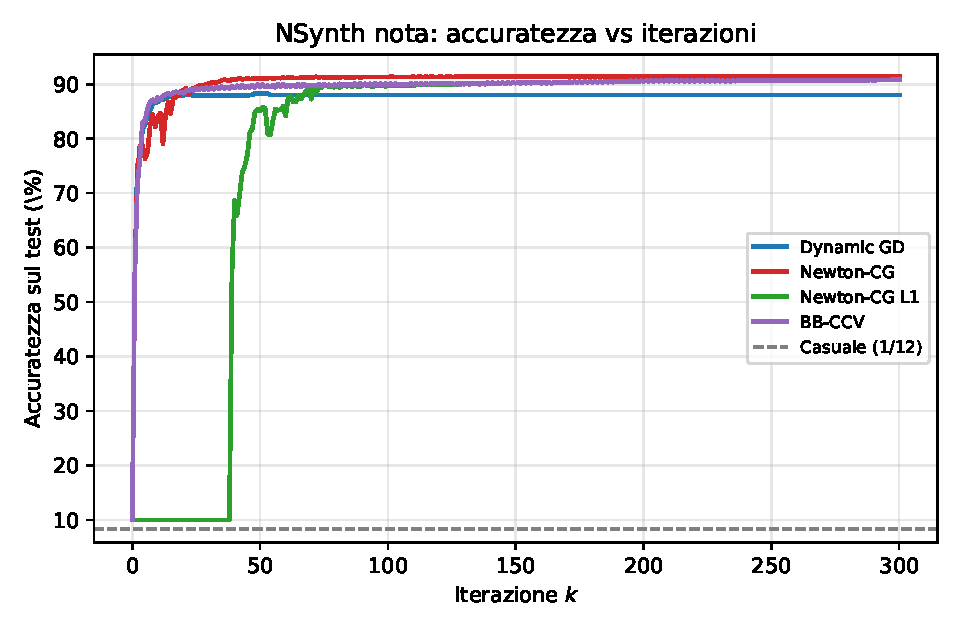
\includegraphics[width=0.8\textwidth]{figure_nsynth_nota/nota_accuracy.pdf}
\caption{Accuratezza sul test NSynth per il riconoscimento della nota in
funzione delle iterazioni $k$. La linea tratteggiata indica la predizione
casuale ($1/12 \approx 8.3\%$).}
\label{fig:nota_acc}
\end{figure}

\begin{figure}[H]
\centering
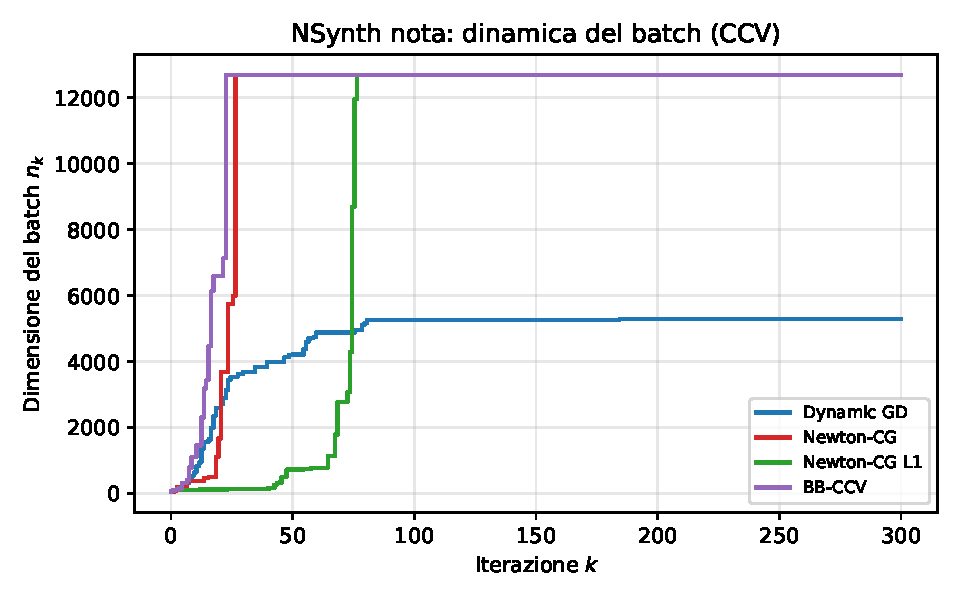
\includegraphics[width=0.8\textwidth]{figure_nsynth_nota/nota_batch.pdf}
\caption{Dimensione del batch $n_k$ per il riconoscimento della nota: anche su
questo compito la CCV aumenta il campione man mano che il gradiente si
riduce.}
\label{fig:nota_batch}
\end{figure}

Tutti i metodi superano di gran lunga la predizione casuale (8.3\%): Dynamic
GD raggiunge l'88.0\%, BB-CCV il 90.8\% e Newton-CG il 91.4\%, in linea con il
solutore di riferimento (L-BFGS di scikit-learn, 91.5\%): il metodo del
secondo ordine converge quindi allo stesso ottimo del solutore standard, con
una differenza inferiore a un decimo di punto percentuale. Il metodo
Newton-CG~$L_1$ ($\nu = 10^{-3}$) raggiunge l'89.8\% e termina entro il
criterio di arresto in 128 iterazioni, azzerando il 51\% dei coefficienti
(146 restano non nulli su 300): la regolarizzazione $L_1$ seleziona le componenti cromatiche
rilevanti per il riconoscimento della nota. Anche su questo compito la CCV
aumenta la dimensione del batch man mano che il gradiente si riduce
(Figura~\ref{fig:nota_batch}). Il solo Dynamic GD fa eccezione: la norma del
suo gradiente ristagna a $\approx 6.8\times10^{-2}$ (non scende mai sotto la
tolleranza di arresto) e perciò la CCV si stabilizza a $n_k = 5\,297$ invece di
spingere il campione fino a $N$. In sintesi, gli stessi algoritmi validati sui
problemi sintetici raggiungono un'accuratezza elevata ($\approx 91\%$) sul
compito musicale del riconoscimento della nota, in linea con il solutore di
riferimento.

\textbf{Riproducibilità.} Tutti gli esperimenti di questa sezione
(estrazione delle features, esecuzione dei quattro metodi, figure e tabelle)
sono riproducibili con il notebook Colab \texttt{nsynth\_nota\_riproduzione},
\url{https://colab.research.google.com/github/Alessandro1040/selezione-dinamica-batch/blob/main/tesi/nsynth/nsynth_nota_riproduzione.ipynb};
il codice è anche disponibile nel repository GitHub
(\url{https://github.com/Alessandro1040/selezione-dinamica-batch}), nella
cartella \texttt{tesi/nsynth/}.

\textbf{Precisione sui valori numerici.} I dati riportati in questa sezione
(accuratezze, norme del gradiente, dimensioni del batch e tempi) si
riferiscono alla run di riferimento eseguita sul computer dell'autore, non a
un'esecuzione in Colab. Il notebook Colab riproduce lo stesso codice con lo
stesso seme casuale (seed 42), ma la riproducibilità non è esatta: gli
algoritmi sono stocastici e i calcoli in virgola mobile dipendono
dall'ambiente di esecuzione (versione di NumPy e libreria BLAS sottostante,
OpenBLAS in Colab contro Accelerate su macOS), per cui piccole differenze di
arrotondamento, accumulate sulle 300 iterazioni, producono valori finali
leggermente diversi. Le differenze sono dell'ordine di qualche decimo di punto
percentuale e non cambiano le conclusioni; i tempi di esecuzione in Colab sono
invece molto più lunghi (minuti, contro pochi secondi sulla macchina locale).

\subsection{Riconoscimento Strumenti}\label{sec:nsynth-net}

Per verificare come si comportano i quattro metodi quando la funzione obiettivo
\textbf{non} è convessa, gli stessi algoritmi dei codici B.1--B.4 sono stati
applicati a una \textbf{rete neurale}, una famiglia di modelli in cui la loss
dipende in modo non lineare dai parametri e non è convessa. Le regole degli
algoritmi (line search di Wolfe, controllo della varianza CCV, gradiente
coniugato, proiezione sull'ortante) restano \emph{invariate}; cambia solo il
modo in cui si calcolano gradiente, loss e prodotto Hessiano--vettore. Nelle
versioni originali questi oggetti si ottengono sommando, per ogni esempio del
batch, il contributo individuale: con una rete di $\approx 234\,000$ parametri
e $N = 12\,678$ esempi questo costo (e la memoria necessaria) rende
l'esecuzione impraticabile su Colab. Si usano quindi versioni \emph{batch},
dette \emph{vettorizzate}: applicano le stesse formule a matrici che
rappresentano l'intero batch in una sola volta, i prodotti $X_b W_1$,
$a_1 W_2$ e $a_2 W_3$ del forward e i prodotti matriciali del passaggio
all'indietro, invece di ripetere il calcolo in un ciclo per ogni esempio
(come definito nella Sezione~\ref{sec:nsynth}). La corrispondenza con le
versioni per-esempio è verificata numericamente (errori dell'ordine di
$10^{-15}$).

L'implementazione è organizzata in un piccolo numero di \textbf{funzioni} che
si richiamano tra loro: la Figura~\ref{fig:nn_funzioni} ne mostra la mappa
completa, mentre le Figure~\ref{fig:nn_features}--\ref{fig:nn_hess} mostrano
il dettaglio di ciascuna, (ingressi $\to$ uscite) e le
formule esatte implementate. I nomi coincidono con quelli del notebook Colab
\texttt{nsynth\_net\_riproduzione}, così gli schemi si confrontano
direttamente con il codice.
\begin{figure}[H]
\centering
\resizebox{0.94\textwidth}{!}{%
\begin{tikzpicture}[
  node distance=2.0cm and 3.0cm,
  every node/.style={font=\small},
  io/.style={
    draw=gray!60, fill=gray!8, rounded corners=3pt,
    text width=3.8cm, align=center, minimum height=1.0cm,
    inner sep=5pt
  },
  box/.style={
    draw=coverblue, fill=coverblue!6, rounded corners=3pt,
    text width=3.8cm, align=center, minimum height=1.0cm,
    inner sep=5pt
  },
  fcn/.style={
    draw=coverblue, fill=coverblue!15, rounded corners=3pt,
    text width=3.4cm, align=center, minimum height=1.05cm,
    inner sep=5pt
  },
  arrow/.style={-{Stealth[length=2.5mm]}, thick, color=coverblue},
  call/.style={-{Stealth[length=2.2mm]}, thick, dashed, color=gray!65},
  label/.style={font=\scriptsize, fill=white, inner sep=1.5pt}
]

  % Preparazione dei dati (riga superiore) - coordinate X ampiamente distanziate
  \node[io] (wav) at (-8.0, 5.5) {Clip audio wav\\(note monofoniche, 4~s, 16~kHz)};
  \node[fcn] (feat) at (-2.0, 5.5) {\texttt{estrai\_features}\\[2pt] clip $\to$ vettore $x_i \in \mathbb{R}^{780}$};
  \node[box] (scal) at (4.0, 5.5) {\texttt{RobustScaler}\\[2pt] $X \in \mathbb{R}^{N\times 780}$, $y$};

  % Funzioni nucleo - coordinate X ampiamente distanziate
  \node[fcn] (fwd) at (4.0, 3.0) {\texttt{forward}($w$, $X_b$)\\[2pt] $\to$ \texttt{logits}, $a_1$, $a_2$};
  \node[fcn] (loss) at (-8.0, 0.0) {\texttt{loss\_batch}($w$, $\mathcal{S}$)\\[2pt] $\to J_{\mathcal{S}}(w)$};
  \node[fcn] (grad) at (-3.0, 0.0) {\texttt{grad\_batch}($w$, $\mathcal{S}$)\\[2pt] $\to \nabla J_{\mathcal{S}}(w)$};
  \node[fcn] (ccv) at (3.0, 0.0) {\texttt{ccv\_stats}($w$, $\mathcal{S}$)\\[2pt] $\to (V,\, \|\bar g\|^2)$};
  \node[fcn] (hess) at (8.0, 0.0) {\texttt{hess\_batch}($w$, $\mathcal{H}$, $v$)\\[2pt] $\to \nabla^2 J_{\mathcal{H}}(w)\,v$};

  % Algoritmi e valutazione
  \node[box, text width=11.0cm, minimum height=1.5cm] (algs) at (0.0, -3.5) {Quattro algoritmi (codici B.1--B.4), logica invariata\\[2pt] Dynamic GD, Newton-CG, Newton-CG $L_1$, BB-CCV};
  \node[io] (eval) at (0.0, -6.5) {\texttt{acc\_test}($w$)\\[2pt] accuratezza su test, tabelle, figure};

  % Frecce dati
  \draw[arrow] (wav) -- (feat);
  \draw[arrow] (feat) -- (scal);
  \draw[arrow] (scal) -- (fwd) node[label, midway, right] {$X$, $y$};

  % forward richiamata dai consumatori
  \draw[call] (fwd.south) -- (loss.north) node[label, pos=0.5, above] {richiama \texttt{forward}};
  \draw[call] (fwd.south) -- (grad.north);
  \draw[call] (fwd.south) -- (hess.north);

  % Consumatori -> algoritmi
  \draw[arrow] (loss.south) -- (algs.north) node[label, pos=0.55, left] {Wolfe};
  \draw[arrow] (grad.south) -- (algs.north) node[label, pos=0.55, left] {passo};
  \draw[arrow] (ccv.south) -- (algs.north) node[label, pos=0.55, right] {CCV};
  \draw[arrow] (hess.south) -- (algs.north) node[label, pos=0.55, right] {CG};

  \draw[arrow] (algs.south) -- (eval.north);

\end{tikzpicture}}
\caption{Mappa delle funzioni dell'implementazione vettorizzata. Dalle clip si
estraggono i vettori $x_i$ (Figura~\ref{fig:nn_features}), normalizzati nella
matrice $X$; \texttt{forward} calcola le attivazioni della rete e le quattro
funzioni che la richiamano forniscono agli algoritmi dei codici B.1--B.4
proprio gli oggetti che essi richiedono: la loss per la line search di Wolfe,
il gradiente per il passo, la varianza per la verifica CCV e il prodotto
Hessiano--vettore per il gradiente coniugato; \texttt{acc\_test} valuta infine
la soluzione sul test. Frecce continue: flusso dei dati; frecce tratteggiate:
chiamate tra funzioni.}
\label{fig:nn_funzioni}
\end{figure}

\textbf{Estrazione delle features (audio $\to$ vettore).}
Una clip è un segnale $y \in \mathbb{R}^T$ di 64\,000 campioni a 16~kHz, cioè un
vettore di pressioni d'aria campionate, da cui nessun algoritmo lavora
direttamente. La funzione \texttt{estrai\_features} lo converte in un vettore
$x_i \in \mathbb{R}^{780}$ di statistiche che riassumono \emph{come suona} la
clip: separa prima il segnale in una parte armonica $y_h$ (il tono) e una
percussiva $y_p$ (gli attacchi), poi calcola su $y_h$ sei famiglie di
descrittori (timbro, altezza, forma spettrale, dinamica) riassumendo ogni
descrittore nel tempo con media e deviazione standard
(Figura~\ref{fig:nn_features}); i valori sono infine normalizzati con un
\texttt{RobustScaler}. Un programmatore non deve conoscere l'audio: basta
sapere che $x_i$ è l'input della rete e che ogni sua componente misura una
caratteristica statistica del suono.
\begin{figure}[H]
\centering
\resizebox{0.88\textwidth}{!}{%
\begin{tikzpicture}[
  node distance=2.0cm and 2.0cm,
  every node/.style={font=\small},
  io/.style={draw=gray!60, fill=gray!8, rounded corners=3pt, text width=3.8cm, align=center, minimum height=1.0cm, inner sep=5pt},
  box/.style={draw=coverblue, fill=coverblue!6, rounded corners=3pt, text width=3.6cm, align=center, minimum height=1.0cm, inner sep=5pt},
  feat/.style={draw=coverblue, fill=coverblue!15, rounded corners=3pt, text width=3.4cm, align=center, minimum height=1.5cm, inner sep=5pt},
  arrow/.style={-{Stealth[length=2.5mm]}, thick, color=coverblue},
  label/.style={font=\scriptsize, fill=white, inner sep=1.5pt}
]

  % Segnale e separazione
  \node[io] (y) at (0, 8.5) {Clip wav\\(4~s, 16~kHz): $y \in \mathbb{R}^{T}$ con $T=64\,000$ campioni};
  \node[box] (hpss) at (0, 6.0) {Separazione armonico-percussiva: $\operatorname{hpss}(y)$\\[2pt] $y_h$ = tono (armonica), \quad $y_p$ = attacchi (percussiva)};

  % Riga 1
  \node[feat] (mel) at (-8.0, 2.8) {\textbf{Mel-spettrogramma}\\[1pt] $S=\operatorname{mel}(y_h)$, 96 bande,\\[1pt] dB, $\Delta$, $\Delta^2$ nel tempo;\\[1pt] media e dev.\ std $\to$ \textbf{384}};
  \node[feat] (mfcc) at (0.0, 2.8) {\textbf{MFCC}\\[1pt] $\operatorname{mfcc}(y_h)$: 40 coeff.\ cepstrali\\[1pt] $+ \Delta$ nel tempo;\\[1pt] media e dev.\ std $\to$ \textbf{160}};
  \node[feat] (cqt) at (8.0, 2.8) {\textbf{CQT}\\[1pt] $|CQT(y_h)|$: 84 bins log-frequenza\\[1pt] in dB;\\[1pt] media e dev.\ std $\to$ \textbf{168}};

  % Riga 2
  \node[feat] (ton) at (-8.0, -2.8) {\textbf{Tonnetz}\\[1pt] $\operatorname{tonnetz}(y_h)$: note\\[1pt] in cerchio di quinte;\\[1pt] media e dev.\ std $\to$ \textbf{12}};
  \node[feat] (spet) at (0.0, -2.8) {\textbf{Contrasto e chroma}\\[1pt] $\operatorname{contrast}(y_h)$ (7 bande),\\[1pt] $\operatorname{chroma}(y_h)$ (12 note);\\[1pt] media e dev.\ std $\to$ \textbf{38}};
  \node[feat] (din) at (8.0, -2.8) {\textbf{Forma spettrale e dinamica}\\[1pt] centroid, bandwidth, rolloff,\\[1pt] flatness, zero-crossing (10); onset,\\[1pt] rms, energie, centroide (8) $\to$ \textbf{18}};

  % Concatenazione e normalizzazione
  \node[io] (concat) at (0, -6.8) {Vettore delle feature: $x_i \in \mathbb{R}^{780}$\\[2pt] $384 + 160 + 168 + 12 + 38 + 18$};
  \node[box] (scaler) at (0, -9.5) {\texttt{RobustScaler} (quantili 5--95), clip a $[-10,10]$\\[2pt] $\to$ riga normalizzata di $X \in \mathbb{R}^{N\times 780}$};

  % Frecce
  \draw[arrow] (y) -- (hpss);
  \draw[arrow] (hpss) -- (mel) node[label, midway, left] {$y_h$};

  \draw[arrow] (mel) -- (mfcc) node[label, midway, above] {concat.};
  \draw[arrow] (mfcc) -- (cqt) node[label, midway, above] {concat.};
  \draw[arrow] (cqt) -- (din) node[label, midway, right] {concat.};
  \draw[arrow] (din) -- (spet) node[label, midway, below] {concat.};
  \draw[arrow] (spet) -- (ton) node[label, midway, below] {concat.};
  \draw[arrow] (ton) -- (ton.south |- concat.north) -- (concat.north);

  \draw[arrow] (concat) -- (scaler);

\end{tikzpicture}}
\caption{\texttt{estrai\_features}: da clip audio a vettore di feature. Il
segnale $y$ è separato in armonica ($y_h$) e percussiva ($y_p$); sei famiglie
di descrittori calcolati su $y_h$ (tonnetz, spettrale e dinamica anche su $y$)
producono medie e deviazioni standard nel tempo, concatenate nel vettore
$x_i \in \mathbb{R}^{780}$ (le cifre indicano le dimensioni di ogni blocco);
infine \texttt{RobustScaler} normalizza le colonne sui quantili 5--95 e i
valori sono limitati a $[-10, 10]$. Le frecce etichettate \emph{concat.}
indicano che i blocchi, calcolati indipendentemente, sono concatenati
nell'ordine mostrato.}
\label{fig:nn_features}
\end{figure}
\textbf{Forward della rete.}
La rete è una funzione $f_w$ che trasforma il batch $X_b \in \mathbb{R}^{m\times 780}$
in un vettore di punteggi per le 10 famiglie strumentali, alternando
trasformazioni affini e attivazioni non lineari $\tanh$: $z_l$ è l'ingresso
dello strato $l$, $a_l = \tanh(z_l)$ la sua uscita, e l'ultimo strato produce
i \emph{logits}, che la softmax convertirà in probabilità. I parametri sono
raccolti nel vettore $w = [W_1; b_1; W_2; b_2; W_3; b_3]$ di
$\approx 234\,000$ valori (Figura~\ref{fig:nn_forward}); la funzione restituisce
anche le attivazioni $a_1, a_2$, che servono alla backpropagation.

\begin{figure}[H]
\centering
\resizebox{0.6\textwidth}{!}{%
\begin{tikzpicture}[
  node distance=1.2cm and 2.0cm,
  every node/.style={font=\small},
  io/.style={draw=gray!60, fill=gray!8, rounded corners=3pt, text width=4.6cm, align=center, minimum height=0.9cm, inner sep=4pt},
  box/.style={draw=coverblue, fill=coverblue!6, rounded corners=3pt, text width=4.6cm, align=center, minimum height=0.9cm, inner sep=4pt},
  arrow/.style={-{Stealth[length=2.5mm]}, thick, color=coverblue},
  call/.style={-{Stealth[length=2.2mm]}, thick, dashed, color=gray!65},
  label/.style={font=\scriptsize, fill=white, inner sep=1.5pt}
]

  \node[io, text width=6.2cm] (sig) {\texttt{forward}($w$, $X_b$)\\[2pt] $\to$ (\texttt{logits}, $a_1$, $a_2$), \quad $X_b \in \mathbb{R}^{m\times 780}$};

  \node[box, below=of sig] (l1) {Strato 1\\[2pt] $z_1 = X_b W_1 + b_1$, \quad $a_1 = \tanh(z_1)$\\[1pt] $W_1 \in \mathbb{R}^{780\times 256}$};
  \node[box, below=of l1] (l2) {Strato 2\\[2pt] $z_2 = a_1 W_2 + b_2$, \quad $a_2 = \tanh(z_2)$\\[1pt] $W_2 \in \mathbb{R}^{256\times 128}$};
  \node[box, below=of l2] (l3) {Strato 3\\[2pt] $\mathrm{logits} = a_2 W_3 + b_3$\\[1pt] $W_3 \in \mathbb{R}^{128\times 10}$};
  \node[io, below=of l3] (out) {Uscite: \texttt{logits} (per la softmax),\\[1pt] $a_1$, $a_2$ (per la backpropagation)};

  \node[io, right=2.0cm of l2, text width=4.6cm, minimum height=3.2cm] (w) {Parametri\\[2pt] $w = [W_1; b_1; W_2; b_2; W_3; b_3]$\\[1pt] $\approx 234\,000$ valori};

  \draw[arrow] (sig) -- (l1);
  \draw[arrow] (l1) -- (l2);
  \draw[arrow] (l2) -- (l3);
  \draw[arrow] (l3) -- (out);

  \draw[call] (w.north west) -- (l1.east) node[label, midway, above] {$W_1, b_1$};
  \draw[call] (w.west) -- (l2.east) node[label, midway, above] {$W_2, b_2$};
  \draw[call] (w.south west) -- (l3.east) node[label, midway, above] {$W_3, b_3$};

\end{tikzpicture}}
\caption{Funzione \texttt{forward} (architettura della rete): tre trasformazioni
affini intervallate dall'attivazione $\tanh$, con le dimensioni delle matrici;
$w$ è l'intero vettore dei parametri, da cui ogni strato legge i propri pesi
$W_l$ e bias $b_l$. I logits sono le uscite grezze dell'ultimo strato.}
\label{fig:nn_forward}
\end{figure}

\textbf{Loss sul batch.}
La funzione \texttt{loss\_batch} restituisce la perdita media sul
sottocampione $\mathcal{S}$, $J_\mathcal{S}(w) = -\frac{1}{m}\sum_{i\in\mathcal{S}}\log
p_{y_i} + \frac{\lambda}{2}\sum_{l=1}^{3}\|W_l\|_F^2$: le probabilità $p$ si
ottengono con la softmax dai logits della \texttt{forward}, e la
regolarizzazione $L_2$ (con $\lambda = 10^{-4}$) è applicata solo alle matrici
dei pesi $W_l$, non ai bias. La Figura~\ref{fig:nn_loss} riassume i passaggi.

\begin{figure}[H]
\centering
\resizebox{0.72\textwidth}{!}{%
\begin{tikzpicture}[
  node distance=0.8cm and 1.2cm,
  every node/.style={font=\small},
  io/.style={draw=gray!60, fill=gray!8, rounded corners=3pt, text width=5.2cm, align=center, minimum height=1.0cm, inner sep=5pt},
  box/.style={draw=coverblue, fill=coverblue!6, rounded corners=3pt, text width=5.2cm, align=center, minimum height=1.0cm, inner sep=5pt},
  arrow/.style={-{Stealth[length=2.5mm]}, thick, color=coverblue},
  label/.style={font=\scriptsize, fill=white, inner sep=1.5pt}
]

  \node[io, text width=6.4cm] (sig) at (0, 4.5) {\texttt{loss\_batch}($w$, $\mathcal{S}$)\\[2pt] $\to J_\mathcal{S}(w) \in \mathbb{R}$, \quad $m = |\mathcal{S}|$ esempi\\[1pt] $X_b = X[\mathcal{S}]$, \quad $Y_b = Y[\mathcal{S}]$};

  % Passi in fila
  \node[box] (fwd) at (-6.0, 2.0) {Logits dalla \texttt{forward}\\[2pt] $(\mathrm{logits}, \cdot, \cdot) = \texttt{forward}(w, X_b)$};
  \node[box] (sm) at (0.0, 2.0) {Softmax stabile (shift del massimo)\\[2pt] $P_{ic} = \dfrac{e^{\,z_{ic} - \max_{c'} z_{ic'}}}{\sum_{c'} e^{\,z_{ic'} - \max_{c'} z_{ic'}}}$};
  \node[box] (ce) at (6.0, 2.0) {Cross-entropia media\\[2pt] $-\dfrac{1}{m}\sum_{i=1}^{m} \log P_{i, Y_{b,i}}$};

  % Regolarizzazione e uscita
  \node[box] (reg) at (0.0, -0.8) {Regolarizzazione $L_2$ (solo pesi, $\lambda = 10^{-4}$)\\[2pt] $\dfrac{\lambda}{2}\bigl(\|W_1\|_F^2 + \|W_2\|_F^2 + \|W_3\|_F^2\bigr)$};
  \node[io] (out) at (0.0, -3.2) {Uscita: $J_\mathcal{S}(w)$ = cross-entropia $+$ regolarizzazione\\[2pt] usata dalla line search di Wolfe};

  \draw[arrow] (sig) -- (fwd);
  \draw[arrow] (fwd) -- (sm);
  \draw[arrow] (sm) -- (ce);
  \draw[arrow] (ce) -- (out) node[label, pos=0.25, above] {$+$};
  \draw[arrow] (reg) -- (out);

\end{tikzpicture}}
\caption{Funzione \texttt{loss\_batch}: logits dalla \texttt{forward}, softmax
stabile, cross-entropia media sul batch e regolarizzazione $L_2$ sui pesi;
l'uscita è la somma dei due contributi.}
\label{fig:nn_loss}
\end{figure}
\textbf{Gradiente del batch.}
Per minimizzare la loss serve il gradiente rispetto ai parametri. Lo si calcola
con la \textbf{backpropagation}: dopo il forward si definisce l'errore
$\delta = (P - Y_b)/m$ tra le probabilità $P$ e la codifica one-hot $Y_b$
delle classi vere, e lo si propaga all'indietro attraverso i tre strati usando
la derivata di $\tanh$, che vale $1 - a^2$; a ogni peso si somma il contributo
di regolarizzazione $\lambda W_l$. Il risultato è la media dei gradienti
individuali, $\nabla J_\mathcal{S}(w) = \frac{1}{m}\sum_{i\in\mathcal{S}}\nabla\ell(w;i)$,
calcolata però in un solo passaggio matriciale sull'intero batch
(Figura~\ref{fig:nn_grad}).
\begin{figure}[H]
\centering
\resizebox{0.78\textwidth}{!}{%
\begin{tikzpicture}[
  node distance=1.2cm and 1.5cm,
  every node/.style={font=\small},
  io/.style={draw=gray!60, fill=gray!8, rounded corners=3pt, text width=4.8cm, align=center, minimum height=0.95cm, inner sep=4pt},
  box/.style={draw=coverblue, fill=coverblue!6, rounded corners=3pt, text width=4.8cm, align=center, minimum height=0.95cm, inner sep=4pt},
  arrow/.style={-{Stealth[length=2.5mm]}, thick, color=coverblue},
  label/.style={font=\scriptsize, fill=white, inner sep=1.5pt}
]

  % Passi iniziali
  \node[io, text width=6.2cm] (sig) at (0, 6.8) {\texttt{grad\_batch}($w$, $\mathcal{S}$)\\[2pt] $\to \nabla J_\mathcal{S}(w)$};
  \node[box] (fwd) at (0, 4.8) {Forward e probabilità\\[2pt] $(\mathrm{logits}, a_1, a_2) = \texttt{forward}(w, X_b)$, \; $P = \mathrm{softmax}(\mathrm{logits})$};
  \node[box] (err) at (0, 2.8) {Errore di output\\[2pt] $\delta = (P - Y_b)/m$ \quad ($Y_b$ = one-hot delle classi)};

  % Backpropagation (tre strati in fila)
  \node[box] (b3) at (-7.0, 0.0) {Strato 3\\[2pt] $dW_3 = a_2^{\top}\delta$, \; $db_3 = \delta^{\top}\mathbf{1}$};
  \node[box] (b2) at (0.0, 0.0) {Strato 2\\[2pt] $\delta_2 = (\delta\, W_3^{\top}) \odot (1 - a_2^2)$\\[1pt] $dW_2 = a_1^{\top}\delta_2$, \; $db_2 = \delta_2^{\top}\mathbf{1}$};
  \node[box] (b1) at (7.0, 0.0) {Strato 1\\[2pt] $\delta_1 = (\delta_2 W_2^{\top}) \odot (1 - a_1^2)$\\[1pt] $dW_1 = X_b^{\top}\delta_1$, \; $db_1 = \delta_1^{\top}\mathbf{1}$};

  % Regolarizzazione e uscita (distanziati ulteriormente)
  \node[box] (reg) at (0, -2.5) {Regolarizzazione (sui pesi)\\[2pt] $dW_l \leftarrow dW_l + \lambda W_l$ \qquad ($l = 1, 2, 3$)};
  \node[io, text width=6.2cm] (out) at (0, -5.5) {Uscita: $\nabla J_\mathcal{S}(w) = \bigl[dW_1;\, db_1;\, dW_2;\, db_2;\, dW_3;\, db_3\bigr]$\\[2pt] $= \dfrac{1}{m}\sum_{i\in\mathcal{S}} \nabla\ell(w; i)$ \quad ($1 - a^2$ = derivata di $\tanh$)};

  \draw[arrow] (sig) -- (fwd);
  \draw[arrow] (fwd) -- (err);
  \draw[arrow] (err) -- (b3) node[label, midway, above] {indietro};
  \draw[arrow] (b3) -- (b2);
  \draw[arrow] (b2) -- (b1);
  \draw[arrow] (b1) -- (reg);
  \draw[arrow] (reg) -- (out);

\end{tikzpicture}}
\caption{Funzione \texttt{grad\_batch}: backpropagation vettorizzata.
L'errore $\delta$ tra probabilità e one-hot è propagato all'indietro con la
derivata di $\tanh$ ($1-a^2$); a ogni matrice dei pesi si somma $\lambda W_l$.
Il risultato coincide con la media dei gradienti per-esempio del codice B.1.}
\label{fig:nn_grad}
\end{figure}
\textbf{Varianza per-esempio per la CCV.}
La condizione di controllo della varianza (codice B.1) richiede la varianza
campionaria dei gradienti individuali sul batch corrente. In forma esatta essa
vale $V = \frac{\sum_i\|g_i\|^2 - n_k\|\bar g\|^2}{n_k - 1}$: per calcolarla
non serve materializzare la matrice $(n_k \times D)$ dei gradienti individuali
(che richiederebbe $n_k \cdot D$ valori, troppi per la memoria di Colab), basta
accumulare la somma dei quadrati delle norme $\sum_i\|g_i\|^2$ calcolando i
gradienti a blocchi di 32 esempi. Il valore ottenuto è \emph{identico} a quello
del codice B.1. La Figura~\ref{fig:nn_ccv} riassume la funzione
\texttt{ccv\_stats} e la sua dipendenza da \texttt{grad\_batch} e
\texttt{per\_example\_sq\_norms}.

\begin{figure}[H]
\centering
\resizebox{0.72\textwidth}{!}{%
\begin{tikzpicture}[
  node distance=0.8cm and 1.2cm,
  every node/.style={font=\small},
  io/.style={draw=gray!60, fill=gray!8, rounded corners=3pt, text width=5.2cm, align=center, minimum height=1.0cm, inner sep=5pt},
  box/.style={draw=coverblue, fill=coverblue!6, rounded corners=3pt, text width=5.2cm, align=center, minimum height=1.0cm, inner sep=5pt},
  arrow/.style={-{Stealth[length=2.5mm]}, thick, color=coverblue},
  label/.style={font=\scriptsize, fill=white, inner sep=1.5pt}
]

  \node[io, text width=6.4cm] (sig) at (0, 4.2) {\texttt{ccv\_stats}($w$, $\mathcal{S}$, \texttt{chunk}=32)\\[2pt] $\to (V, \|\bar g\|^2)$};

  \node[box] (gbar) at (-4.0, 2.0) {Gradiente medio\\[2pt] $\bar g = \texttt{grad\_batch}(w, \mathcal{S})$};
  \node[box] (loop) at (4.0, 2.0) {\texttt{per\_example\_sq\_norms}\\[2pt] a blocchi di 32 esempi:\\[1pt] $s_2 \leftarrow s_2 + \sum_{i\in B}\|g_i\|^2$};
  \node[box] (var) at (-4.0, -0.8) {Varianza per-esempio esatta\\[2pt] $V = \dfrac{s_2 - m\,\|\bar g\|^2}{m - 1}$, \quad $m=|\mathcal{S}|$};
  \node[io] (out) at (0, -3.2) {Uscita: $(V, \|\bar g\|^2)$ per la verifica CCV\\[2pt] $\dfrac{V}{m} \le \theta^2 \|\bar g\|^2$};

  \draw[arrow] (sig) -- (gbar);
  \draw[arrow] (gbar) -- (loop) node[label, midway, above] {norme $\|G_B\|^2$};
  \draw[arrow] (gbar) -- (var);
  \draw[arrow] (loop) -- (var) node[label, midway, right] {$s_2$};
  \draw[arrow] (var) -- (out);

\end{tikzpicture}}
\caption{Funzione \texttt{ccv\_stats}: gradiente medio dal \texttt{grad\_batch},
somma dei quadrati delle norme per-esempio calcolata a blocchi di 32 esempi
(per non materializzare la matrice $n_k \times D$) e combinazione nella
formula esatta della varianza campionaria; l'uscita alimenta la verifica CCV
del codice B.1.}
\label{fig:nn_ccv}
\end{figure}

\textbf{Prodotto Hessiano--vettore.}
Il metodo Newton-CG richiede, a ogni iterazione del gradiente coniugato, il
prodotto tra l'Hessiana della loss media sul sottocampione $\mathcal{H}_k$ e un
vettore $v$. Poiché l'Hessiana della media è la media delle Hessiane, questo
prodotto coincide con la media dei prodotti per-esempio; \texttt{hess\_batch}
lo calcola con un'unica chiamata di differenziazione automatica sulla funzione
$f(w') = J_{\mathcal{H}_k}(w')$ (Figura~\ref{fig:nn_hess}). Per contenere il
costo si pone $\gamma = 0$ nel criterio di arresto del CG (la stima della
varianza degli Hessiani per-esempio sarebbe proibitiva) e si usa $\alpha = 1$
come passo iniziale delle line search, come nel resto della tesi.

\begin{figure}[H]
\centering
\resizebox{0.7\textwidth}{!}{%
\begin{tikzpicture}[
  node distance=0.8cm and 1.2cm,
  every node/.style={font=\small},
  io/.style={draw=gray!60, fill=gray!8, rounded corners=3pt, text width=5.2cm, align=center, minimum height=1.0cm, inner sep=5pt},
  box/.style={draw=coverblue, fill=coverblue!6, rounded corners=3pt, text width=5.2cm, align=center, minimum height=1.0cm, inner sep=5pt},
  arrow/.style={-{Stealth[length=2.5mm]}, thick, color=coverblue}
]

  \node[io, text width=6.4cm] (sig) at (0, 4.5) {\texttt{hess\_batch}($w$, $\mathcal{H}$, $v$)\\[2pt] $\to \nabla^2 J_\mathcal{H}(w)\,v$, \quad $\mathcal{H} \subseteq \mathcal{S}$};

  \node[box] (f) at (-6.0, 2.0) {Loss media sul sottocampione\\[2pt] $f(w') = J_\mathcal{H}(w')$};
  \node[box] (hvp) at (0.0, 2.0) {Differenziazione automatica\\[2pt] $\texttt{hessian\_vector\_product}(f)$\\[1pt] in una sola chiamata};
  \node[box] (eq) at (6.0, 2.0) {Equivalenza per-esempio\\[2pt] $\nabla^2 J_\mathcal{H}(w)\,v$\\[1pt] $= \frac{1}{|\mathcal{H}|}\sum_{i\in\mathcal{H}}\nabla^2\ell(w;i)\,v$};

  \node[io] (out) at (0, -1.8) {Vettore per il gradiente coniugato\\[2pt] $\gamma = 0$ nel criterio di arresto, $\alpha = 1$ nelle line search};

  \draw[arrow] (sig) -- (f);
  \draw[arrow] (f) -- (hvp);
  \draw[arrow] (hvp) -- (eq);
  \draw[arrow] (eq) -- (out);
  \draw[arrow] (hvp) -- (out);

\end{tikzpicture}}
\caption{Funzione \texttt{hess\_batch}: il prodotto Hessiano--vettore sul
sottocampione $\mathcal{H}$ è calcolato definendo la loss media $f$ e
chiamando \texttt{hessian\_vector\_product} una sola volta; il valore coincide
con la media dei prodotti per-esempio.}
\label{fig:nn_hess}
\end{figure}

Il notebook \texttt{nsynth\_net\_riproduzione}, disponibile nella cartella
\texttt{tesi/nsynth/} del repository, implementa fedelmente le funzioni qui
descritte: la cella di validazione interna verifica numericamente, su un
piccolo batch, che le funzioni batch coincidano con le versioni per-esempio
(errori inferiori a $10^{-8}$ sul gradiente, sulla loss e sulla
varianza CCV, e inferiori a $10^{-6}$ sul prodotto
Hessiano--vettore), garantendo che l'uso delle versioni vettorizzate non
altera i risultati degli algoritmi.

\textbf{Risultati dell'esperimento.}
I quattro metodi sono stati applicati alla rete con $200$ iterazioni, seed $42$,
batch iniziale $128$ e soglia CCV $\theta=0{,}3$; per contenere il costo delle
iterazioni la dimensione del batch è stata limitata a $n_k\le 2048$ (senza
limite la CCV tenderebbe a far crescere il batch verso l'intero training set,
$N = 12\,678$). La Tabella~\ref{tab:nsynth_net} riporta per ogni metodo
l'accuratezza sul test set ($4\,096$ clip), la norma del gradiente finale, la
dimensione del batch finale, il tempo di addestramento e, per il metodo con
regolarizzazione $L_1$, il numero di coefficienti non nulli. La
Figura~\ref{fig:nsynth_net_acc} mostra l'accuratezza di test al variare
dell'iterazione $k$, mentre la Figura~\ref{fig:nsynth_net_batch} mostra la
dinamica della dimensione del batch $n_k$ scelta dal controllo CCV.

\begin{table}[H]
\centering
\caption{Rete neurale su NSynth: risultati dei quattro metodi (200 iterazioni,
cap del batch a 2048, seed 42; tempi su Apple M5).}
\label{tab:nsynth_net}
\begin{tabular}{lccccc}
\toprule
Metodo & Acc. test & $\|\nabla J(w)\|_2$ & Batch fin. & Tempo (s) & Coeff. $\neq 0$\\
\midrule
Dynamic GD      & 96.9\% & $4.1\times10^{-1}$ & 2048 & 148.8 & ---\\
Newton-CG       & 99.2\% & $3.0\times10^{-2}$ & 2048 & 210.2 & ---\\
Newton-CG $L_1$ & 97.3\% & $7.0\times10^{-1}$ & 2048 & 196.9 & $58\,412/234\,122$\\
BB-CCV          & 96.2\% & $8.4\times10^{-2}$ & 2048 & 216.9 & ---\\
\bottomrule
\end{tabular}
\end{table}

\begin{figure}[H]
\centering
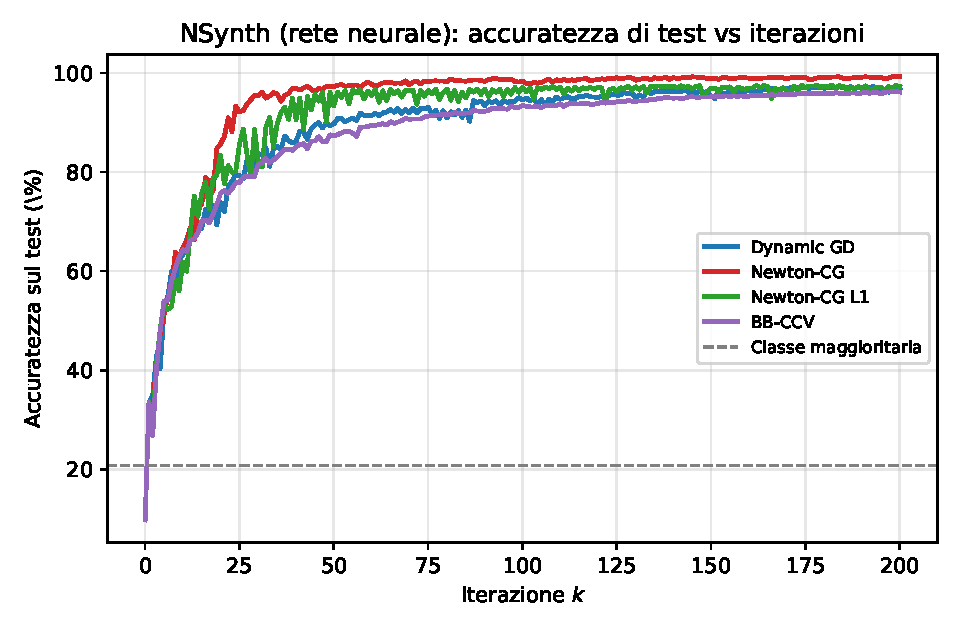
\includegraphics[width=0.85\textwidth]{figure_nsynth_net/nsynth_accuracy_net.pdf}
\caption{NSynth (rete neurale): accuratezza sul test set in funzione delle
iterazioni per i quattro metodi; la linea tratteggiata indica la frequenza
della classe maggioritaria (20.8\%).}
\label{fig:nsynth_net_acc}
\end{figure}

\begin{figure}[H]
\centering
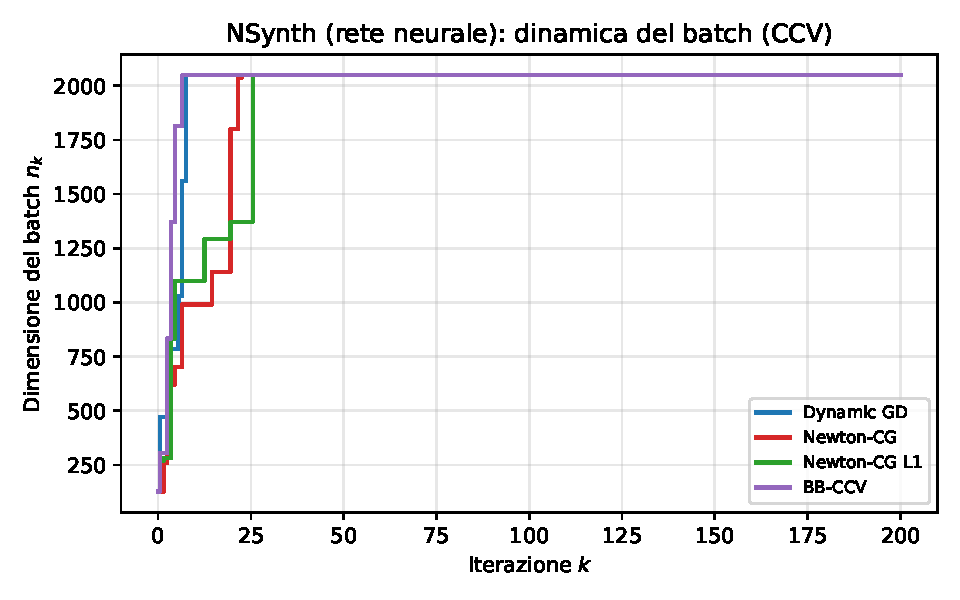
\includegraphics[width=0.85\textwidth]{figure_nsynth_net/nsynth_batch_net.pdf}
\caption{NSynth (rete neurale): dimensione del batch $n_k$ scelta dal controllo
CCV a ogni iterazione per i quattro metodi (tetto a 2048).}
\label{fig:nsynth_net_batch}
\end{figure}

Il codice completo è disponibile nel notebook Colab
\texttt{nsynth\_net\_riproduzione},
\url{https://colab.research.google.com/github/Alessandro1040/selezione-dinamica-batch/blob/main/tesi/nsynth/nsynth_net_riproduzione.ipynb};
un secondo notebook, \texttt{nsynth\_net\_test},
\url{https://colab.research.google.com/github/Alessandro1040/selezione-dinamica-batch/blob/main/tesi/nsynth/nsynth_net_test.ipynb},
carica i pesi addestrati e lo scaler e verifica i modelli su clip reali con le
etichette vere: per una clip scelta (per indice o nome) stampa la famiglia vera
e le predizioni dei quattro metodi --- ad esempio la clip
\texttt{keyboard\_electronic\_078-053-050} del test set è classificata come
\emph{keyboard} da tutti i metodi con probabilità superiore al 99\% --- e
permette inoltre di caricare un proprio file audio e di ascoltare le clip.
L'intero repository, con script, figure e note operative, è disponibile su
\url{https://github.com/Alessandro1040/selezione-dinamica-batch}.

\textbf{Riproducibilità.} Tutti gli esperimenti di questa sezione (estrazione
delle features, addestramento dei quattro metodi, figure e tabelle) sono
riproducibili eseguendo dall'inizio il notebook Colab
\texttt{nsynth\_net\_riproduzione} indicato sopra: le celle successive al
download di NSynth (split validation e test) estraggono le features, eseguono i
quattro metodi con i parametri dichiarati in questa sezione e generano le
figure e la tabella in formato LaTeX con gli stessi valori qui riportati; la
cella di validazione interna garantisce che le versioni vettorizzate delle
funzioni non alterino i risultati rispetto alle versioni per-esempio dei codici
B.1--B.4.

\textbf{Precisione sui valori numerici.} I dati riportati in questa sezione
(accuratezze, norme del gradiente, dimensioni del batch e tempi) si riferiscono
alla run di riferimento eseguita sul computer dell'autore, non a un'esecuzione
in Colab. Il notebook Colab riproduce lo stesso codice con lo stesso seme
casuale (seed 42), ma la riproducibilità non è esatta: gli algoritmi sono
stocastici e i calcoli in virgola mobile dipendono dall'ambiente di esecuzione
(versione di NumPy e libreria BLAS sottostante, OpenBLAS in Colab contro
Accelerate su macOS), per cui piccole differenze di arrotondamento, accumulate
sulle 200 iterazioni, producono valori finali leggermente diversi. Le
differenze sono dell'ordine di qualche decimo di punto percentuale e non
cambiano le conclusioni; i tempi di esecuzione in Colab sono invece molto più
lunghi (decine di minuti, contro i pochi minuti della macchina locale).






\begin{thebibliography}{9}

\bibitem{engel2017}
J.~Engel, C.~Resnick, A.~Roberts, S.~Dieleman, M.~Norouzi, D.~Eck, and
K.~Simonyan,
``Neural audio synthesis of musical notes with WaveNet autoencoders,''
in \textit{Proceedings of the 34th International Conference on Machine
Learning (ICML)}, 2017.

\end{thebibliography}

\end{document}
